\documentclass[italian, a4paper, 10pt, twocolumn]{../../style/lab_unige}
% \usepackage[a4paper, margin=1.25cm, footskip=0.25in]{geometry}

\usepackage[utf8]{inputenc}
\usepackage[T1]{fontenc}

\usepackage[italian]{babel}

\usepackage[bookmarksopen=true, citebordercolor={0 1 0}, linkbordercolor={1 0 0}, urlbordercolor={0 1 1}]{hyperref}
\usepackage[numbered]{bookmark}

\usepackage{graphicx}
\graphicspath{{../fig/}}
\usepackage{array}
\usepackage{tabulary}
\usepackage{booktabs}

% FOUNDAMENTAL
\usepackage{../../style/custom}

\usepackage{physics}

\usepackage{breqn}
\usepackage{cuted}
\usepackage{txfonts} %%%%%%%%% Times Font package

%% Define ref types
\newcommand{\reftab}[1]{Tab. {\ref{#1}}}%
\newcommand{\reffig}[1]{Fig. {\ref{#1}}}%
\newcommand{\refeqn}[1]{({\ref{#1})}}%
%%
\setlength{\columnsep}{6mm}
\begin{document}

\twocolumn[
  \begin{@twocolumnfalse}
    
    \title{
    	Misura dell'accelerazione di gravità con un pendolo semplice
    }
    \author{
      Eugenio Dormicchi\textsuperscript{1},  
      Riccardo Pizzimbone\textsuperscript{1}, 
      Mattia Sotgia\textsuperscript{1}
    }

    \date{
      \textsuperscript{1}Gruppo C03, Esperienza di laboratorio n. 4\\%% !! cambiare numero esperienza 
      %\textsuperscript{2}In presenza in laboratorio per la presa dati\\
    	% Università degli Studi di Genova, Dipartimento di Fisica.\\
    	Presa dati–– 
    	22 dicembre 2020, 15:00– 18:00; Analisi dati–– 
    	11 gennaio 2021
    }
    \maketitle
    
    \begin{abstract}
      
      \textit{Obiettivo– }
      Determinare, sfruttando il moto di un pendolo e considerandolo nel regime delle piccole oscillazioni,
      il valore dell'accelerazione di gravità $g$.
      \textit{Metodi– }
      Consideriamo un pendolo, nelle sue piccole oscillazioni, di cui possiamo 
      misurare la lunghezza $L=L_{0}+L_{CM}$. Cronometriamo $N=10$ oscillazioni per più
      ripetizioni, trovando così periodi $\bar{T_{i}}=T_{10}/N$, rispettivi alle Lunghezze
      $L_{i}$. Facendo variare la lunghezza, misuriamo nuovamente il periodo
      del pendolo. 
      \textit{Risultati– }
      Sfruttando gli strumenti di calcolo otteniamo dal fit lineare i valori di $g\pm\varepsilon g$.
      \textit{Conclusione– }
      Confrontando statisticamente i dati, otteniamo una compatibilità degli stessi con il valore teorico 
      $g_{t}=(9.8056\pm0.0001_{\text{stat}}) \text{ m/s}^{2}$.
    \end{abstract}
    \vspace{2em}
    \end{@twocolumnfalse}
]

	%%%% CORPO DEL TESTO
  %%%% CORPO DEL TESTO

  \section{Obiettivo}

  Lo scopo dell'esperienza è di ricavare dal moto oscillatorio di un pendolo, considerato nel regime delle 
  piccole oscillazioni\footnote{Come osserviamo più avanti, gli angoli 
  individuati dalle oscillazioni del pendoli sono $<15^\circ\approx0.26\text{ rad}$.} 
  e approssimato a pendolo semplice, il valore dell'accelerazione di gravità $g$, valutando come 
  trascurabile la massa del filo del pendolo, che in tutti e tre gli apparati considerati ha massa inferiore
  sensibilità della bilancia.
  \\

  Da qui in poi ci riferiremo con A a Eugenio Dormicchi, con B a Riccardo Pizzimbone e con C a
  Mattia Sotgia.

  \section{Strumentazione}
  Di seguito elenchiamo la strumentazione utilizzata da ogni studente, a cui ci riferiamo secondo la 
  nomenclatura sopra indicata.

  \subsection{Strumentazione A}
  Cilindro di acciaio inox.: massa $(8.50\pm0.01)\times10^{-1}$ kg, altezza $(1.430\pm0.01)\times10^{-1}$ m, 
  diametro $(7.630\pm0.005)\times10^{-2}$ m;\\
  Filo di tessuto inestensibile di massa trascurabile;\\
  Metro a nastro: portata 3 m, sensibilità $1\times10^{-3}$ m;\\
  Cronometro: sensibilità 0.1 s;\\
  Bilancia elettronica da cucina: portata 3 kg; incertezza = sensibilità $1\times10^{-3}$ kg;\\
  Struttura per sospendere il pendolo ad una altzza $h$ (barra di trazione e moschettone).\\

  \subsection{Strumentazione B}
  Pallina di natale cava con un foro tappato una volta riempita d'acqua: diametro $(3.4\pm0.3)\times10^{-2}$ m,
  massa $(1.68\pm0.01)\times10^{-1}$ kg;\\
  Filo di nylon estensibile\footnote{per minimizzare il fattore di allungamento del filo, quest'ultimo è 
  rimasto una notte in tensione.};\\
  Gancio fisso per sospendere il pendolo;\\
  Metro a nastro: portata 1.5 m, sensibilità $1\times10^{-3}$ m;\\
  Flessometro: portata 3 m, sensibilità $1\times10^{-3}$ m;\\
  Bilancia elettronica da cucina: portata 3 kg; incertezza = sensibilità $1\times10^{-3}$ kg;\\
  Cronometro: sensibilità 0.01 s;\\ 
  Struttura per sospendere il pendolo ad una altzza $h$ (parte inferiore letto a castello).\\


  \newpage

  \subsection{Strumentazione C}
  Pallina di natale sferica piena di sale: diametro $(39.05\pm0.05)$ mm\\
  Filo di nylon estensibile\footnote{La lunghezza del filo viene presa quando questo è già in tensione,
  quindi il fattore di allungamento viene incluso già nella misurazione.};\\
  Flessometro fissato di fianco al pandolo, tale da misurarne la lunghezza nella condizione di equilibrio
  stabile: portata 2 m, sensibilità $1\times10^{-3}$ m;\\
  Cronometro: sensibilità 0.01 s;\\
  Bialncia elettronica: portata 5 kg, sensibilità $1\times10^{-3}$ kg;\\
  Struttura per sospendere il pendolo ad una altzza $h$ (mensola posta ad una altezza di 2.34 m da terra).\\

  \section{Metodi}
  Misuriamo con il cronometro la durata di 10 oscillazioni di un pendolo, ottenendo quindi il periodo 
  di una oscillazione completa $T=T_{10}/10$. Eseguiamo la stessa misura 10 volte per 5 lunghezze 
  diverse ($L_{i}$) del pendolo. Possiamo perciò procedere con uno studio statistico dei dati, 
  ricavandoci il periodo medio ($\bar{T}$) e il relativo Errore Standard $\varepsilon_{N}T$.
  \\

  % NOTE DI CARATTERE GENERALE
  Tutte le misure sono riportate in unità del Sistema internazionale (SI). \\
  Si fa spesso riferimento anche alla regola del $3\sigma$, con la quale si vuole intendere la volontà 
  di trasformare un errore di tipo massimo in errore statistico, e quindi considerando il valore vero
  con una probabilità statistica del $3\sigma\approx99.73\%$ di probabilità del dato vero.\\
  %% MAGARI AGGIUNGERE COMMENTO SU QUANTE CIFRE SI CONSIDERANO E COME APPROSSIMIAMO I VALORI %%
  I valori riportati sono stati approssimati tenendo conto di alcune convenzioni prese. Si 
  approssima l'errore ad una cifra significativa se tale cifra è $\geqslant3$, altrimenti se tale
  cifra è 1 o 2 allora si considerano due cifre significative. Considerando quindi le posizioni decimali
  significative dell'errore si approssima per eccesso il valore numerico della grandezza. 


  
  
  \begin{figure}[t!]
    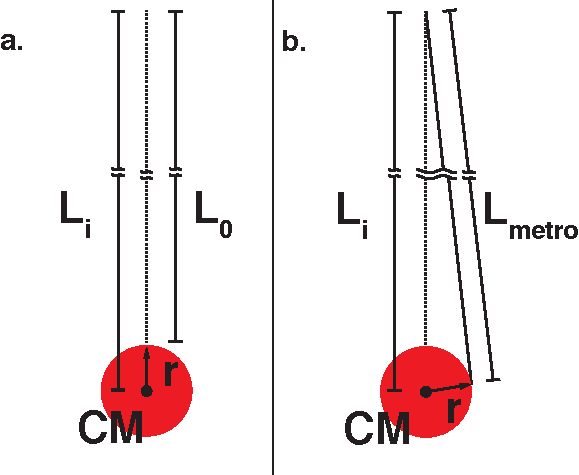
\includegraphics[width=\linewidth]{pendulum_simple.pdf}
    \caption{Due diversi modelli di pendolo. \textbf{a.} Pendolo che illustra come sono state prese le misure di 
    $L_{i}$ da A e B, ovvero considerando la lunghezza $L_{0}$ del filo solo e poi considerando la lunghezza $r$,
    ovvero sfruttando la particolare simmetria del corpo (simile per A che ha considerato una simmetria 
    cilindrica), sommando i due valori. \textbf{b.} Il metodo di misura di $L_{i}$ per i dati C, come descritto
    nel par. \ref{section:data_analysys_c}, sfrutta il fatto che la misura è effettuata quando il pendolo è già
    in tensione massima, ovvero nel punto di equilibrio stabile, e poi sfruttando la costuzione geometrica che si
    crea tra $r$, $L_{\text{metro}}$ e $L_{i}$.}
    \label{fig:pendulum}
  \end{figure}

  \subsection{Caratterizzazione apparato sperimentale}
  \label{section:car_apparato_gen}
  
  \subsubsection{Apparato sperim. A} % Eugenio Dormicchi
  Precedentemente alla costruzione dell’apparato sperimentale sono state misurate: la massa del cilindro 
  con la bilancia elettronica, l’altezza del cilindro con il metro a nastro e il diametro del solido con 
  il calibro.

  Una barra di trazione viene fermata ad una altezza di 2.10 m. Ad essa viene fissato il filo inestensibile 
  tramite un moschettone. Al filo è fissato il cilindro tramite un gancio. Al solido è incollata lungo 
  l’asse con il  'blue tack' una punta utile per traguardare il pendolo. Al di sotto del pendolo veniva 
  posto un foglio con una linea centrale che facilitava la presa delle oscillazioni. Il foglio in questione 
  era posto a sua volta sopra un quaderno munito di un elastico da cui si faceva partire il pendolo. 

  Dopo aver effettuato 10 misure delle oscillazioni il filo veniva ridotto così da far variare la lunghezza
   del pendolo. Si ripeteva poi il procedimento precedentemente descritto posizionando il 
  foglio e il quaderno sopra delle scatole piane. 

  La misura della lunghezza dell’apparato oscillante veniva calcolata misurando con il metro dalla parte 
  superiore del moschettone alla base del cilindro ($L_{0}$ vedi \reffig{fig:pendulum}a.). 
  Successivamente si sottraeva metà dell’altezza del cilindro ottenendo così la lunghezza $L_{i}$ del pendolo
  dal moschettone al centro di massa (CM, da qui in poi). 

  \subsubsection{Apparato sperim. B} % Riccardo Pizzimbone
  È fissato un gancio a una struttura stabile alta circa 1.7 m, sul gancio è stata legata l’estremità di 
  un filo e all’altra estremità si trova una pallina di Natale piena d’acqua (fino all’orlo, cosicché il 
  CM non si sposti durante le oscillazioni); quest’ultima è attaccata al filo tramite un nodo su un gancetto
  in plastica (di massa trascurabile e lunghezza presa in considerazione durante le misurazioni) già 
  presente sulla pallina. 
  
  Il gancio è posizionato in modo tale che il pendolo costruito 
  dal filo e dal corpo non urti nulla con nessuna delle sue componenti. Al di sotto del pendolo è stato 
  fissato a terra un foglio, su questo sono stati segnati il punto di equilibrio stabile (da qua in avanti 
  tale punto verrà riferito come punto $P_{\text{e}}$) e il punto da cui far partire le oscillazioni che 
  sarà sempre uguale per ogni altezza (la distanza tra il punto $P_{\text{e}}$ e quello d'inizio 
  oscillazione è $\sim5.7\times10^{-2}$m). Per mantenere costante il punto d'inizio oscillazione a ogni 
  quota sperimentata sono stati posizionati oggetti stabili e alti sul foglio in corrispondenza del punto 
  in cui è stata fatta la prima oscillazione. Per far cambiare quota al corpo sospeso è stato accorciato il 
  filo arrotolandolo intorno al gancio. 
  
  Prima di costruire il pendolo 
  son stati misurati massa, con una bilancia elettronica da cucina, circonferenza e diametro della pallina, 
  con un metro a nastro; posizionato il pendolo è stata misurata la lunghezza del filo in massima estensione 
  per ogni quota con un flesso metro. 
  


  \subsubsection{Apparato sperim. C}
  \label{section:app_s_c}
  Ho misurato con il calibro il diametro della sfera.
  Ho misurato poi la massa del solido con la bilancia elettronica.

  Alla mensola era fissato un supporto di legno dove, tramite una pinza, era fissato il filo di nylon, fatto
  passare in modo che fosse libero di scorrere nell'anello della pinza. Un capo del filo era poi legato alla
  sfera, l'altro capo era fissato a un moschettone che permetteva di allungare o accorciare la lunghezza del 
  pendolo. A una distanza di $\sim1\times10^{-1}$ m dalla posizione $P_{\text{e}}$ del pendolo era
  posizionato un'asta verticale parallela al filo del pendolo (nella condizione di equilibrio), che potesse
  indicare una posizione di partenza fissa (x) per le oscillazioni. 

  Il supporto del pendolo era tale da permettere di poter fissare nello stesso punto del filo del pendolo 
  anche il flesso metro, facendo sì che la misure della lunghezza potessero essere prese già con il filo in 
  tensione, includendo così ogni effetto di possibile elongazione del filo di nylon. Il metro veniva posto 
  a fianco del pendolo in stato di equilibrio, e si prendeva come misura ($L_{\text{metro}}$) il punto di 
  tangenza tra la pallina e il metro. 
  In questo modo non è necessario ricavare separatamente il CM della sfera.

  Bisogna considerare che però la lunghezza qui misurata non è $L_{i}$, poiché è presente un angolo tra l'asse
  del pendolo e la direzione lungo cui avviene la misura. Conoscendo però il raggio della pallina 
  ($\text{diametro}/2=r$) sappiamo che la direzione di misura è tangente alla sfera, quindi perpendicolare al 
  raggio, quindi $L_{i}=\sqrt{r^{2}+(L_{\text{metro}})^{2}}$. 

  \begin{table*}[t!]
    \footnotesize
    \centering
    \caption{Set dati A: ricavati come descritto in \textit{\ref{section:presa_dati} Presa dati}, $E_{r\%}$ 
    indica invece l'errore relativo ottenuto da $\varepsilon x_{i}/\bar{x_{i}}$.}
    \label{tab:A}
    % \setlength{\tabcolsep}{2.385\tabcolsep}
    \setlength{\tabcolsep}{1.93\tabcolsep}
    \begin{tabular}{lccccccccc}
      \hline\hline\\[-1.5ex]
        & \multicolumn{3}{c}{Lunghezza totale pendolo (m)} & \multicolumn{3}{c}{Periodo singola osc.$^{\text{a}}$ (s)}  & \multicolumn{3}{c}{Periodo al quadrato singola osc.$^{\text{a}}$ ($\text{s}^{2}$)} \\[+0.5ex] 
        & $L_{i}$ & $\varepsilon L_{i}$ & $E_{r\%}$        & $\bar{T}_{i}$  & $\varepsilon\bar{T}_{i}$                  & $E_{r\%}$ & $\bar{T}_{i}^{2}$ & $\varepsilon\bar{T}_{i}^{2}$ & $E_{r\%}$     \\[+0.5ex] \hline \\[-1.5ex]
      1 & 1.8835  & $1.2\times10^{-3}$  & $0.06\%$         & 2.752          & $6\times10^{-3}$                          & $0.22\%$  & 7.574             & $3 \times10^{-2}$            & $0.4\%$      \\[+0.5ex]
      2 & 1.6175  & $1.2\times10^{-3}$  & $0.07\%$         & 2.551          & $6\times10^{-3}$                          & $0.24\%$  & 6.508             & $3 \times10^{-2}$            & $0.5\%$      \\[+0.5ex]
      3 & 1.4585  & $1.2\times10^{-3}$  & $0.08\%$         & 2.424          & $6\times10^{-3}$                          & $0.25\%$  & 5.876             & $2.9 \times10^{-2}$          & $0.5\%$      \\[+0.5ex]
      4 & 1.1495  & $1.2\times10^{-3}$  & $0.10\%$         & 2.147          & $6\times10^{-3}$                          & $0.28\%$  & 4.610             & $2.6 \times10^{-2}$          & $0.6\%$      \\[+0.5ex]
      5 & 0.9135  & $1.2\times10^{-3}$  & $0.13\%$         & 1.922          & $6\times10^{-3}$                          & $0.3\%$   & 3.694             & $2.3 \times10^{-2}$          & $0.6\%$      \\[+0.5ex] 
      \hline \\[-1.5ex]
    \end{tabular}
    \raggedright
    \bfseries Note:\\
    \normalfont
    \textsuperscript{a} Per l'incertezza sul periodo, poiché la sensibilità del cronometro era di $0.1$ s e 
    $0.1/(10\sqrt{3})$, ovvero la sensibilità sperimentale 'staticizzata' è maggiore degli Errori Std. 
    ($\varepsilon \bar{T}_{i}$), si è considerato come valore di $\varepsilon \bar{T}_{i}$ il valore 
    $0.1/(10\sqrt{3})=6\times10^{-3}$. Analogamente $\varepsilon \bar{T}_{i}^{2}$ è stato calcolato a partire 
    dal valore di $0.1/(10\sqrt{3})=6\times10^{-3}$.
  \end{table*}

  \begin{table*}[t!]
    \footnotesize
    \centering
    \caption{Set dati B, come sopra.}
    \label{tab:B}
    % \setlength{\tabcolsep}{2.408\tabcolsep}
    \setlength{\tabcolsep}{1.985\tabcolsep}
    \begin{tabular}{lccccccccc}
      \hline\hline\\[-1.5ex]
        & \multicolumn{3}{c}{Lunghezza totale pendolo (m)}  & \multicolumn{3}{c}{Periodo singola osc. (s)}          & \multicolumn{3}{c}{Periodo al quadrato singola osc. ($\text{s}^{2}$)} \\[+0.5ex] 
        & $L_{i}$ & $\varepsilon L_{i}$ & $E_{r\%}$         & $\bar{T}_{i}$  & $\varepsilon\bar{T}_{i}$ & $E_{r\%}$ & $\bar{T}_{i}^{2}$ & $\varepsilon\bar{T}_{i}^{2}$ & $E_{r\%}$     \\[+0.5ex] \hline \\[-1.5ex]
      1 & 1.6260  & $6\times10^{-4}$    & $0.06\%$          & 2.529          & $4\times10^{-3}$         & $0.16\%$  & 6.394             & $2.0\times10^{-2}$           & $0.3\%$       \\[+0.5ex]
      2 & 1.4680  & $6\times10^{-4}$    & $0.07\%$          & 2.405          & $4\times10^{-3}$         & $0.17\%$  & 5.785             & $1.8\times10^{-2}$           & $0.3\%$       \\[+0.5ex]
      3 & 1.2960  & $6\times10^{-4}$    & $0.08\%$          & 2.271          & $3\times10^{-3}$         & $0.13\%$  & 5.157             & $1.4\times10^{-2}$           & $0.27\%$      \\[+0.5ex]
      4 & 1.1450  & $6\times10^{-4}$    & $0.09\%$          & 2.124          & $5\times10^{-3}$         & $0.24\%$  & 4.512             & $2.2\times10^{-2}$           & $0.5\%$       \\[+0.5ex]
      5 & 1.0210  & $6\times10^{-4}$    & $0.10\%$          & 2.007          & $5\times10^{-3}$         & $0.25\%$  & 4.028             & $2.1\times10^{-2}$           & $0.5\%$       \\[+0.5ex]
      \hline
    \end{tabular}
  \end{table*}

  \begin{table*}[t!]
    \footnotesize
    \centering
    \caption{Set dati C; per questi dati il trattamento è stato lievemente diverso da come sono stati trattati 
    i dati in \reftab{tab:A} e \reftab{tab:B}, in quanto, come indicato nella sezione \textit{
    \ref{section:app_s_c}}, la  $i$-esima lunghezza $L_{i}$ è presa secondo la formula 
    $L_{i}=\sqrt{(d/2)^{2}+(L_{\text{metro}})^{2}}$, e quindi $\varepsilon L_{i}$, calcolato a partire da 
    $\varepsilon d=\Delta d/\sqrt{3}$ e $\varepsilon L_{\text{metro}}=\Delta L_{\text{metro}}/\sqrt{3}$, 
    trovati secondo la regola del $3\sigma$. I calcoli eseguiti sono riportati nel paragrafo
    \textit{\ref{section:data_analysys_c} Trattamento dati C}.
    Sono inoltre stati presi valori su sette lunghezze del pendolo.}
    \label{tab:C}
    % \setlength{\tabcolsep}{2.408\tabcolsep}
    \setlength{\tabcolsep}{1.985\tabcolsep}
    \begin{tabular}{lccccccccc}
      \hline\hline\\[-1.5ex]
        & \multicolumn{3}{c}{Lunghezza totale pendolo (m)}  & \multicolumn{3}{c}{Periodo singola osc. (s)}               & \multicolumn{3}{c}{Periodo al quadrato singola osc. ($\text{s}^{2}$)} \\[+0.5ex] 
        & $L_{i}$ & $\varepsilon L_{i}$ & $E_{r\%}$         & $\bar{T}_{i}$  & $\varepsilon\bar{T}_{i}$ & $E_{r\%}$ & $\bar{T}_{i}^{2}$ & $\varepsilon\bar{T}_{i}^{2}$ & $E_{r\%}$     \\[+0.5ex] \hline \\[-1.5ex]
      1 & 1.9401  & $6\times10^{-4}$    & $0.03\%$          & 2.788          & $5\times10^{-3}$         & $0.18\%$  & 7.772             & $2.8\times10^{-2}$           & $0.4\%$       \\[+0.5ex] % punto originario 1 
      2 & 1.7541  & $6\times10^{-4}$    & $0.03\%$          & 2.647          & $2\times10^{-3}$         & $0.09\%$  & 7.006             & $1.3\times10^{-2}$           & $0.18\%$      \\[+0.5ex] % punto originario 2
      3 & 1.5991  & $6\times10^{-4}$    & $0.04\%$          & 2.523          & $4\times10^{-3}$         & $0.14\%$  & 6.366             & $1.8\times10^{-2}$           & $0.3\%$       \\[+0.5ex] % punto originario 3
      4 & 1.5081  & $6\times10^{-4}$    & $0.04\%$          & 2.461          & $3\times10^{-3}$         & $0.11\%$  & 6.056             & $1.4\times10^{-2}$           & $0.26\%$      \\[+0.5ex] % punto originario 6
      5 & 1.4131  & $6\times10^{-4}$    & $0.04\%$          & 2.382          & $3\times10^{-3}$         & $0.10\%$  & 5.673             & $1.2\times10^{-2}$           & $0.21\%$      \\[+0.5ex] % punto originario 4
      6 & 1.3142  & $6\times10^{-4}$    & $0.04\%$          & 2.299          & $4\times10^{-3}$         & $0.16\%$  & 5.284             & $1.6\times10^{-2}$           & $0.3\%$       \\[+0.5ex] % punto originario 5
      7 & 1.1652  & $6\times10^{-4}$    & $0.05\%$          & 2.148          & $3\times10^{-3}$         & $0.15\%$  & 4.613             & $1.3\times10^{-2}$           & $0.3\%$       \\[+0.5ex] % punto originario 7
      \hline
    \end{tabular}
  \end{table*}

  \subsection{Presa dati}
  \label{section:presa_dati}
  Portiamo il pendolo ad una certa distanza (x) dalla posizione $P_{\text{e}}$ e cerchiamo di mantenere 
  fissa tale posizione per tutte le misure, 
  lasciamo il corpo e facciamo simultaneamente partire il cronometro. Contiamo $N=10$ oscillazioni, alla 
  fine delle quali fermiamo il cronometro, ottenendo il valore $T_{1\times10}$ (ovvero 10 oscillazioni 
  per la lunghezza $L_{1}$). Ripetiamo il procedimento, riportando il pendolo alla posizione x per 10 
  volte, alla lunghezza del pendolo $L_{1}$ (dove $L_{1}$ è la lunghezza fino al CM). 

  Otteniamo quindi il valore del singolo periodo $T_{1}^{(n)}$, ovvero la misura \textit{n}-esima 
  (sono eseguite per ogni lunghezza 10 misure del periodo) del periodo per la 
  lunghezza $L_{1}$, come $T_{1}^{(n)}=T_{1\times10}/10$. 
  Consideriamo ora il valore medio del periodo per la lunghezza $L_{1}$, 
  $\bar{T}_{1}=\left(\sum_{n=1}^{10}T_{1}^{(n)}\right)/10$.
  Calcoliamo anche l'Errore Standard $\varepsilon_{(10)}T_{1}$ con la formula:
  \[
    \varepsilon_{10}T_{1}=\frac{S_{10}}{\sqrt{10}} \text{  dove (}S_{10}\text{ è la Dev. Std. adattata)}
  \]

  Ricaviamo inoltre anche l'errore statistico sulla lunghezza $L_{1}$, sfruttando la regola del $3\sigma$, 
  ottenendo quindi $\varepsilon L_{1}=\Delta L/\sqrt{3}$, dove $\Delta L$ è l'errore massimo di $L_{1}$ 
  (ovvero l'errore propagato sul calcolo di $L_{1}$ dal punto dove è fissato il pendolo al CM).
  
  Ripetiamo le $10\text{ oscillazioni}\times10\text{ volte}$ per 5 lunghezze $L_{i}$ diverse. Per ogni 
  lunghezza eseguiamo i calcoli riportati sopra, ottenendo i valori riportati nelle tabelle \reftab{tab:A} 
  e \reftab{tab:B}.

  Abbiamo ricavato poi a partire da $\bar{T}_{i}$ il valore di $\bar{T}_{i}^{2}=(\bar{T}_{i})^{2}$ con relativo
  errore ricavato come $\varepsilon \bar{T}_{i}^{2}=2\cdot \bar{T}_{i} \cdot \varepsilon \bar{T}_{i}$. Questi valori
  torneranno utili per eseguire il fit lineare dei dati. 
  
  \subsubsection{Trattamento statistico dati C}
  \label{section:data_analysys_c}
  Come osservato in \ref{section:app_s_c} Apparato sperim. C, la $i$-esima lunghezza $L_{i}$ è definita 
  a partire da $L_{\text{metro}}^{(i)}\pm\varepsilon L_{\text{metro}}$ (indichiamo $L_{\text{metro}}^{(i)}$ 
  con $L_{\text{m}}^{(i)}$) e $d\pm\varepsilon d$ secondo la relazione:
  \[L_{i}=\sqrt{\left(L_{\text{m}}^{(i)}\right)^{2}+\frac{d^{2}}{4}}\]
  con errore statistico ricavato come:
  
  \begin{strip}
    \[\varepsilon L_{i}=
    \sqrt{\left(\frac{2\cdot L_{\text{m}}^{(i)}}{2\sqrt{\left(L_{\text{m}}^{(i)}\right)^{2}+\frac{d^{2}}{4}}}\right)^{2} \varepsilon L_{\text{m}}^{2}
                +\left(\frac{\frac{1}{2}\cdot d}{2\sqrt{\left(L_{\text{m}}^{(i)}\right)^{2}+\frac{d^{2}}{4}}}\right)^{2} \varepsilon d^{2}
    }\]
  \end{strip}

  dove gli errori $\varepsilon L_{\text{m}}^{(i)}$ e $\varepsilon d$ sono ricavati secondo la regola del $3\sigma$,
  ottenendo quindi $\varepsilon L_{\text{m}}=\Delta L_{\text{m}}/\sqrt{3}$  e $\varepsilon d=\Delta d/\sqrt{3}$.
  I valori sono poi riportati in \reftab{tab:C}.

  Questo diverso trattamento è dovuto alla differente presa dati che è stata effettuata sfruttando la particolare 
  geometria dell'apparato sperimentale (\textit{cfr:} par. \ref{section:app_s_c}).


  \begin{figure*}
    \centering
    \includegraphics[width=0.325\linewidth]{dati_a_lin.pdf}
    \includegraphics[width=0.325\linewidth]{dati_b_lin.pdf}
    \includegraphics[width=0.325\linewidth]{dati_c_lin.pdf}
    \includegraphics[width=0.325\linewidth]{dati_a_nonlin.pdf}
    \includegraphics[width=0.325\linewidth]{dati_b_nonlin.pdf}
    \includegraphics[width=0.325\linewidth]{dati_c_nonlin.pdf}
    \caption{\textbf{Sopra:} Grafici linearizzati ottenuti dal periodo al quadrato del pendolo in funzione 
    della sua lunghezza. Sono presentati i dati di tre set diversi, con i relativi indicatori statistici 
    del $\chi^{2}$, dei gradi di libertà ($ndf$) e della probabilità del $\chi^{2}$. \textbf{Sotto:}
    Si è provato anche ad effettuare il fit di una funzione non lineare considerando il periodo semplice 
    $T_{i}$ in funzione di $L_{i}$, osservando un andamento parabolico, che rispecchia la teoria.}
    \label{fig:all_graphs}

  \end{figure*}

  \begin{table*}[t]
    \footnotesize
    \centering
    \caption{Valori dell'accelerazione di gravità $g$, espressi in (ms$^{-2}$), ottenuti dal fit eseguito dai dati 
    A, B, C, considerando il valore ottenuto considerando un offset $\neq0$ su $L_{i}$. Inoltre aggiungiamo anche 
    i valori ottenuti dai dati A+B+C. Il trattamento spcifico di A+B+C è molto simile ai singoli dati, ma viene ripreso
    nel par. \ref{par:multiplot}.}
    \label{tab:results}
    \begin{tabulary}{\linewidth}{LcCcCcCcC}
      \hline\hline\\[-1.5ex]
                                                                            & \multicolumn{6}{c}{Dati singoli}                                                                                                                                                                                \\[+0.5ex] \cline{2-7} \\[-2.5ex]
                                                                            & \multicolumn{2}{c}{Dati A}                       & \multicolumn{2}{c}{Dati B}                       & \multicolumn{2}{c}{Dati C}                        & \multicolumn{2}{c}{Dati A+B+C\textsuperscript{b}}     \\[+0.5ex] \hline \\[-2.5ex]
      accelerazione di gravità \newline $g\pm\varepsilon g$ (ms$^{-2}$)     & $9.85\pm0.09$ & err. rel. $0.9\%$                & $10.11\pm0.11$ & err. rel. $1.1\%$               & $9.81\pm0.06$ & err. rel. $0.7\%$                 & $9.76\pm0.09$ & err. rel. $0.9\%$                     \\[+2.0ex] \hline \\[-1.5ex]
      Offset\textsuperscript{a} \newline $\delta\pm\varepsilon \delta$ (m)  & \multicolumn{2}{l}{$2\pm5\times10^{-2}\approx0$} & \multicolumn{2}{l}{$6\pm6\times10^{-2}\approx0$} & \multicolumn{2}{c}{$-4\pm4\times10^{-2}\approx0$} & \multicolumn{2}{c}{$-1.6\pm1.1\times10^{-2}\approx0$} \\[+2.0ex] \hline \\[-1.5ex]

    \end{tabulary}
    \raggedright
    \bfseries Note:\\
    \normalfont
    \textsuperscript{a} Consideriamo offset la distanza tra il valore di $L_{0}$ del fit per $T=0$, 
                        ovvero l'eventuale errore di misurazione della $i$-esima lunghezza $L_{i}$,
                        che può aver portato a sovrastimare o sottostimare il valore vero di $L_{i}$.\\
    \textsuperscript{b} Dati ottenuti dal fit complessivo di tutti e tre i set di dati A+B+C (\reffig{fig:multigraph_all_data}).

  \end{table*}


  \subsection{Linearizzazione dei dati}

  Rappresentati i plot dei dati non linearizzati, ovvero rappresentando i valori ottenuti in un grafico 
  $\bar{\text{T}}_{i}\times \text{L}_{i}$, otteniamo i grafici in \reffig{fig:all_graphs} (Sotto), 
  passiamo alla linearizzazione dei valori, per poter valutare statisticamente i dati raccolti, e 
  ottenere un fit lineare \reffig{fig:all_graphs} (Sopra).

  Partendo dall'equazione di un pendolo semplice
  \begin{equation}\label{eqn:periodo_sqrt}
    T=2\pi\sqrt{\frac{L}{g}}
  \end{equation}
  possiamo ottenere una linearizzazione come
  \begin{equation}\label{eqn:periodo_lineare}
    T^{2}=\frac{4\cdot\pi^{2}}{g}\cdot L
  \end{equation}
  e considerando il grafico $\bar{\text{T}}_{i}^{2}\times \text{L}_{i}$, possiamo osservare un rapporto 
  di proporzionalità diretta tra i valori di $\bar{T}_{i}^{2}$ e $L_{i}$, considerando il coefficiente 
  $4\pi^{2}/g$ come una costante k.

  Eseguiamo quindi un fit lineare con una equazione del tipo $\text{Y}=k\text{X}+\delta$ ponendo 
  $\bar{T}_{i}^{2}=\text{Y}$ e $4\pi^{2}/g=k$ e considerando il fattore $\delta$ di offset, ovvero di 
  possibile sovrastima o sottostima della lunghezza $L_{i}$; otteniamo dal fit il valore di $k$ con 
  il suo errore statistico $\varepsilon k$.


  \section{Risultati}
  \label{section:risultati}

  Per eseguire il fit con \verb|root| grazie al programma \verb|graph_all.C| abbiamo considerato un 
  \verb|TF1| dove la funzione è uguale a \refeqn{eqn:periodo_lineare}, dove $g$ è rappresentato come il 
  parametro \verb|p0|, il parametro \verb|p1|, che indicava $\pi$, è impostato con il metodo 
  \verb|TF1::FixParameter()| e l'offset $\delta$ è il parametro \verb|p2|.

  Il programma \verb|graph_all.C| si basa su i file \verb|ed_dati_modifica.dat|, 
  \verb|rp_dati.dat| e \verb|ms_dati.dat|, dove 
  sono trascritti i valori non-linearizzati di \reftab{tab:A}, \reftab{tab:B} e \reftab{tab:C} in formato
  \begin{verbatim}
    L_1 T_1 eL_1 eT_1
    ...
    L_N T_N eL_N eT_N
  \end{verbatim}
  e sui file \verb|ed_dati_lin_modifica.dat|, \verb|rp_dati_lin.dat| e \verb|ms_dati_lin.dat|
  in formato
  \begin{verbatim}
    L_1 T2_1 eL_1 eT2_1
    ...
    L_N T2_N eL_N eT2_N
  \end{verbatim}

  Eseguendo il fit \verb|root| riportava i valori dei parametri \verb|p0|, \verb|p1|, \verb|p2| con i
  rispettivi errori statistici, valori riportati poi in \reftab{tab:results}.

  Calcoliamo inoltre gli errori relativi ($E_{r\%}$) associati a ciascuna grandezza.

  \section{Conclusione}
  Ottenuti i valori di $g\pm\varepsilon g$ e $\delta\pm\varepsilon\delta$ il suo offset procediamo con
  un'analisi critica degli stessi. 

  \subsection{Controlli}

  Osserviamo innanzitutto che per tutti i set di dati raccolti il valore dell'offset è compatibile con zero, 
  che è in accordo con la teoria; questo è anche piuttosto significativo in quanto mostra che le stime delle 
  lunghezze $L_{i}$ sono realistiche.

  Preso come riferimento il valore dell'accelerazione di gravità a Genova il valore 
  $g_{t}=(9.8056\pm0.0001_{\text{stat}})$ m/s$^{2}$, procediamo a confrontare i valori ottenuti di $g$,
  secondo la relazione
  \[
    \left|g_{t}-g\right|<3\sqrt{\varepsilon g_{t}^{2}+\varepsilon g^{2}}
  \]
  ottenendo quindi per i dati A
  \[\left|9.8056-9.85\right|<3\sqrt{0.0001^{2}+0.09^{2}}\approx0.04<0.27\]
  per i dati B\footnote{Nonostante abbiamo detto sopra come trattiamo l'approssimazione dei dati, ci permettiamo
  in questa situazione di ovviare tale regola per sottolineare che i due valori sono tra loro compatibili.}
  \[\left|9.8056-10.11\right|<3\sqrt{0.0001^{2}+0.11^{2}}\approx0.30<0.33\]
  e per i dati C
  \[\left|9.8056-9.81\right|<3\sqrt{0.0001^{2}+0.06^{2}}\approx0.004<0.18\]

  Osserviamo quindi che i valori dei dati A, B e C sono compatibili con il valore $g_{t}$ fornito.

  Applicando la medesima formula osserviamo che i valori di A e B sono compatibili tra loro (0.26<0.43),
  così anche i valori di A e C (0.04<0.32) e anche i valori di B e C (0.30<0.37)\footnotemark[4].

  
  Calcoliamo quindi la miglior stima del valore dell'accelerazione di gravità $g_{*}$
  \[
    g_{*}=\frac{\frac{g_{A}}{\varepsilon g_{A}^{2}}+\frac{g_{B}}{\varepsilon g_{B}^{2}}+\frac{g_{C}}{\varepsilon g_{C}^{2}}}
    {\frac{1}{\varepsilon g_{A}^{2}}+\frac{1}{\varepsilon g_{B}^{2}}+\frac{1}{\varepsilon g_{C}^{2}}}=9.87 \text{ m/s}^{2}
  \]
  con relativo errore
  \[
    \varepsilon g_{*}=\frac{1}{\sqrt{\frac{1}{\varepsilon g_{A}^{2}}+\frac{1}{\varepsilon g_{B}^{2}}+\frac{1}{\varepsilon g_{C}^{2}}}}=0.05\text{ m/s}^{2}
  \]

  \subsection{Possibili errori sistematici}
  
  Come già osservato i valori dell'intercetta (offset $\delta$) sono tutti compatibili con zero. 
  Questo oltre ad essere in perfetto accordo con la teoria implica che i valori di $L_{0}$ misurati 
  tenevano conto della posizione del CM e lo individuavano correttamente.

  Conoscendo lo spostamento dalla posizione $P_{\text{e}}$ al punto da cui sono fatte partire le 
  oscillazioni (chiamiamo questa distanza x, che come detto in par. \ref{section:car_apparato_gen}), e conoscendo $L_{i}$, 
  possiamo ricavare l'angolo $\vartheta_{\text{MAX}}$ di massima oscillazione
  \[
  \vartheta_{\text{max}}=\arctan\left(\frac{x}{L_{\text{min}}}\right)\times\frac{180}{\pi}
  \]
  Otteniamo che $\vartheta_{\text{max, A}}\approx4^\circ$, $\vartheta_{\text{max, B}}\approx3^\circ$ e 
  $\vartheta_{\text{max, C}}\approx5^\circ$, quindi trascurabile rispetto all'approssimazione di piccole 
  oscillazioni in cui consideriamo il pendolo semplice con le formule \refeqn{eqn:periodo_sqrt}.

  I dati raccolti provengono da tre set diversi e tre apparati diversi che utilizzano pendoli con 
  masse e geometrie differenti. Nonostante questo i valori ottenuti dalla precedente analisi dati 
  sono compatibili tra di loro e con il valore $g_{t}$ teorico previsto. Possiamo perciò concludere 
  che la differenza di massa non influisce sul valore di $g$, e quindi come previsto dalla teoria 
  la massa non influenza l'oscillazione del pendolo, purché esso sia considerato in un regime di 
  piccole oscillazioni.

  Si osserva che l'accorciamento della lunghezza del pendolo porta ad alzare rispetto alla quota iniziale il corpo.
  Si potrebbe quindi riflettere che tale variazione di quota potrebbe causare una leggera variazione sul valore 
  di $g$. Tuttavia, considerando la massima escursione di $L_{i}$ che possiamo avere, quelle di A ($\sim1$ m)
  possiamo provare a quantificare la variazione di $g$. Consideriamo $h_{\text{min}}=0$ quando il pendolo presenta la
  massima $L_{i}$ e $h_{\text{max}}=L_{\text{max}}-L_{\text{min}}$. 
  
  Consideriamo la relazione
  \[g=g_{t}\cdot\left(1-\frac{2h}{R_{\text{terra}}}\right)\]
  ricavata sviluppando con Taylor la formula
  \[|g|=G\cdot\frac{M_{\text{terra}}}{\left(R_{\text{terra}+h}\right)^{2}}\]

  Possiamo perciò trovare la variazione $\delta g$ dell'accelerazione di gravità
  \begin{dmath*}
  \delta g=\left|g_{t}\cdot\left(1-\frac{2h_{\text{max}}}{R_{\text{terra}}}\right)-g_{t}\cdot\left(1-\frac{2h_{\text{min}}}{R_{\text{terra}}}\right)\right|=
  \left|2g_{t}\cdot\left(\frac{h_{\text{min}}-h_{\text{max}}}{R_{\text{terra}}}\right)\right|
  \approx3\times10^{-6} \text{m/s}^{2}
  \end{dmath*}

  Osserviamo quindi che la variazione di $g$ "staticizzata" ($\delta g / \sqrt{3}$) è $\ll$ dell'errore che ricaviamo dal fit dei dati.\\


  \begin{figure}[t]
    \includegraphics[width=\linewidth]{multigraph_set_final_v2.pdf}
    \caption{Plot dati A, B e C, con relativo fit non-lineare ottenuto considerando la relazione \refeqn{eqn:periodo_sqrt}
    non linearizzata, e ottenendo quindi il valore di $g$ dal fit.}
    \label{fig:multigraph_all_data}
  \end{figure}
  \paragraph{Multiplot dati A+B+C}\label{par:multiplot}
  Proviamo infine a raggruppare i dati raccolti da A+B+C ed eseguiamo un plot di questo set esteso di dati
  (\reffig{fig:multigraph_all_data}).
  Eseguiamo un fit non-lineare dei dati sfruttando \verb|root| e il programma \verb|multigraph.C|, e una 
  funzione simile al paragrafo \ref{section:risultati}.
  Otteniamo dat fit i parametri \verb|p0|, \verb|p1|, \verb|p2|, con i relativi errori, che vengono trascritti in 
  \reftab{tab:results}.\@
  Osserviamo che il valore di offset ($\delta$) è $\neq0$, ovvero che l'insieme dei dati riporta un leggero scostamento 
  dall'origine. Il valore di $g\pm\varepsilon g$ viene invece compatibile secondo la relazione
  \[\left|9.8056-9.76\right|<3\sqrt{0.0001^{2}+0.09^{2}}\approx0.05<0.27\]
  che quindi conferma ancora la bontà dei dati raccolti.
  
  
  
\end{document}